\chapter{Fundamentação Teórica}
\label{cap:fundamentacao-teorica}

Este capítulo apresenta os fundamentos teóricos que sustentam esta pesquisa. A Seção~\ref{sec:conceitos-fl} introduz os princípios gerais do \gls{fl} e sua arquitetura. A Seção~\ref{sec:tipos-ataques} discute vulnerabilidades e ataques adversariais que motivam este trabalho. Por fim, a Seção~\ref{sec:defesa-agregacao-robusta} apresenta algoritmos de agregação robusta que serão objeto de avaliação experimental.

\section{Conceitos Gerais de Aprendizado Federado}
\label{sec:conceitos-fl}

O \textbf{\gls{fl}} é um paradigma de treinamento distribuído que visa preservar a privacidade dos dados, permitindo que múltiplos clientes, como dispositivos ou instituições, cooperem no treinamento de modelos sem a necessidade de centralizar dados \cite{McMahan2017}. Nesse esquema, cada cliente realiza treinamento local e apenas as atualizações de parâmetros são enviadas ao servidor central para agregação \cite{Moshawrab2023}. Esse método surge como resposta à crescente preocupação com privacidade de dados e desafios de segurança em ambientes distribuídos, além de viabilizar colaboração em cenários com dados sensíveis ou restrições legais \cite{Kairouz2021}.

% O ciclo de vida tradicional do \gls{fl} envolve as seguintes etapas \cite{Moshawrab2023}:
% \begin{enumerate}
%     \item Inicialização do modelo global pelo servidor.
%     \item Treinamento local do modelo nos clientes participantes.
%     \item Envio de gradientes ou parâmetros locais ao servidor.
%     \item Agregação das atualizações recebidas.
%     \item Redistribuição do modelo global atualizado aos clientes.
% \end{enumerate}

% A Figura~\ref{fig:fl-framework} ilustra a arquitetura clássica do \gls{fl}.
No \gls{fl}, o servidor central inicializa um modelo global e o distribui a um subconjunto de clientes participantes. Cada cliente realiza o treinamento local com seus próprios dados e, ao final dessa etapa, envia ao servidor apenas as atualizações do modelo, como gradientes ou parâmetros. Em seguida, o servidor agrega as atualizações recebidas para compor uma nova versão do modelo global e a redistribui aos clientes para a próxima rodada de treinamento \cite{Moshawrab2023}.

Esse processo ocorre em rodadas de comunicação e preserva a privacidade ao manter os dados no dispositivo/organização de origem, compartilhando apenas atualizações do modelo. O algoritmo de agregação atua como o mecanismo central que combina as contribuições locais e define como o conhecimento de cada cliente é incorporado ao modelo global \cite{McMahan2017,Kairouz2021,Yang2019}.

A Figura~\ref{fig:fl-framework} ilustra a arquitetura clássica do \gls{fl}.
\begin{figure}[H]
    \centering
    \caption{Arquitetura geral do \textit{Federated Learning}}
    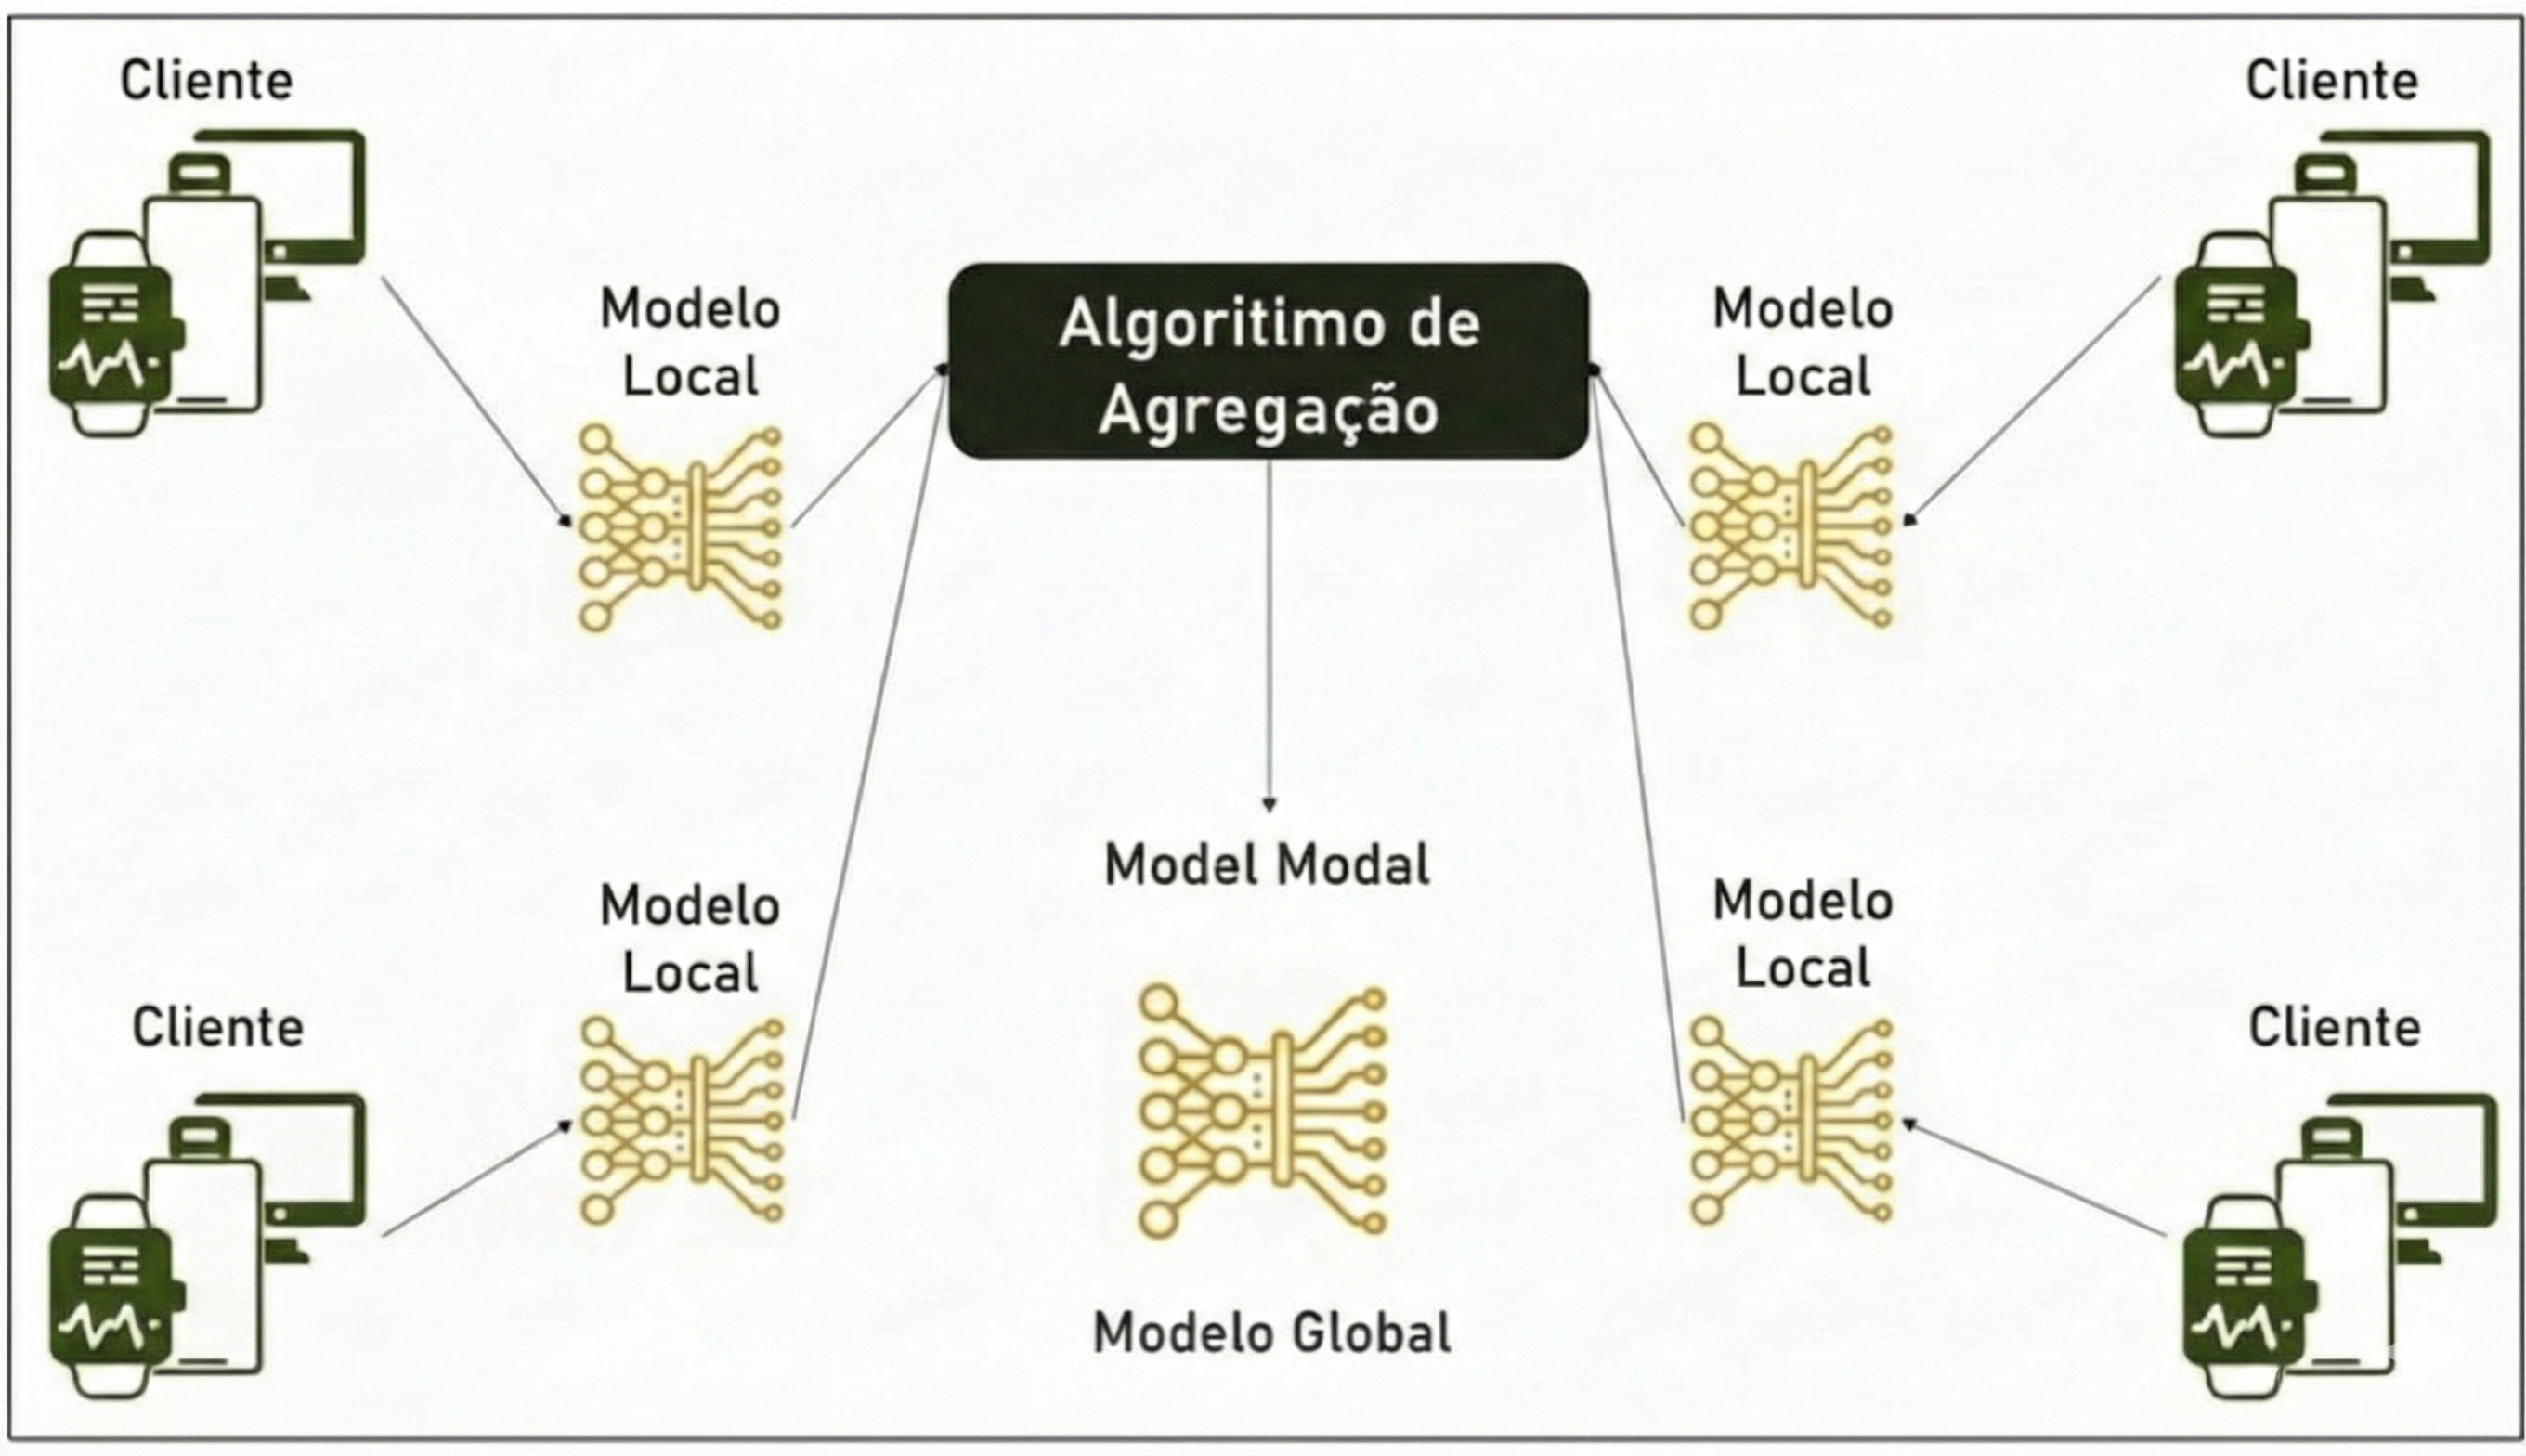
\includegraphics[width=0.8\textwidth]{figuras/electronics-12-02287-g002-550.png}
    \fonte{Adaptado de Moshawrab et al., 2023}
    \label{fig:fl-framework}
\end{figure}

Sob a perspectiva da distribuição dos dados entre os participantes, os principais tipos de \gls{fl} são: horizontal, vertical e por transferência \cite{Bharati2022}.
% O \gls{fl} pode ser classificado de acordo com a forma como os dados estão distribuídos entre os participantes, sendo os principais tipos: horizontal, vertical e por transferência \cite{Bharati2022}.

\begin{itemize}
    \item \textbf{Horizontal, também conhecido como \textit{cross-device}:} ocorre quando diferentes participantes possuem os mesmos tipos de atributos, isto é, o mesmo espaço de características, mas amostras diferentes. Um exemplo clássico é o uso de \gls{fl} para previsão de texto em celulares: milhões de \textit{smartphones} possuem dados próprios de digitação, amostras distintas, mas compartilham o mesmo formato de entrada \cite{McMahan2017,Yang2019}.

    \item \textbf{Vertical, também conhecido como \textit{cross-silo}:} neste caso, os participantes possuem as mesmas amostras, compartilhando certos indivíduos ou entidades, mas cada um detém diferentes características sobre elas. Um exemplo é a colaboração entre bancos e empresas de varejo: ambos possuem registros sobre os mesmos clientes, porém os bancos fornecem informações financeiras e os varejistas, históricos de compras \cite{Zhang2021}.

    \item \textbf{Transferência:} ocorre quando há pouca interseção entre as amostras e ou características dos dados de cada participante. Nesses cenários, utiliza-se \textit{aprendizado por transferência} para mapear diferentes domínios de forma que as contribuições possam ser aproveitadas em tarefas correlatas \cite{Bharati2022}.
\end{itemize}

\subsection{FedAvg e limitações de segurança}
\label{subsec:fedavg-limitacoes}

O \textit{FedAvg}, abreviação de \textit{Federated Averaging}, representa o método de agregação mais fundamental em \gls{fl}. Nele, cada cliente recebe o modelo global, executa treinamento local com seus dados privados e envia apenas os parâmetros atualizados ao servidor \cite{McMahan2017,Yang2019}. O servidor combina essas atualizações por uma média ponderada, atribuindo maior influência aos clientes com conjuntos de dados maiores \cite{Li2020}. Por sua ampla adoção, o \textit{FedAvg} é utilizado como \textit{baseline} em comparação com estratégias robustas \cite{Kairouz2021}.

Apesar de suas vantagens práticas, a simplicidade do \textit{FedAvg} revela vulnerabilidades já discutidas em estudos iniciais e posteriores de segurança em \gls{fl} \cite{Blanchard2017}. A limitação central é não distinguir atualizações legítimas, ainda que heterogêneas, de atualizações deliberadamente manipuladas. Um atacante pode explorar isso enviando parâmetros com magnitudes arbitrariamente grandes, distorcendo a agregação \cite{Tolpegin2020,Bhagoji2019}, ou inserindo comportamentos adversariais específicos que permanecem pouco evidentes em testes convencionais e se manifestam sob gatilhos, como em \textit{backdoors} \cite{Almutairi2024}.

Em ambientes realistas, nos quais a confiança não pode ser totalmente garantida e múltiplos participantes podem ter incentivos conflitantes, a ameaça se torna particularmente severa \cite{Khan2023,Mothukuri2021}. Essas limitações motivam o desenvolvimento de técnicas de agregação robusta que preservem benefícios do \gls{fl} e resistam a ataques adversariais \cite{Chen2023,Xu2024,Sikandar2023}.

\subsection{Heterogeneidade de Dados Non-IID}
\label{subsec:heterogeneidade-noniid}

Um desafio crítico em \gls{fl} é a heterogeneidade natural dos dados entre participantes, fenômeno conhecido como distribuição não \textit{IID}. O termo \textit{IID} significa \textit{Independent and Identically Distributed}, isto é, independente e identicamente distribuído \cite{Zhao2018}. Em cenários realistas, os dados locais dos clientes raramente seguem a mesma distribuição; ao contrário, apresentam padrões e vieses significativamente distintos \cite{Li2020}.

Como exemplo, em um sistema federado para predição de risco cardiológico com colaboração entre hospitais, cada instituição pode atender populações com perfis demográficos e epidemiológicos distintos. Se cada instituição treina apenas com dados locais enviesados e a agregação ocorre via \textit{FedAvg}, o modelo resultante pode não representar adequadamente as populações, degradando desempenho em cenários reais \cite{Zhao2018,Bhagoji2019}.

A heterogeneidade pode retardar a convergência, exigindo mais rodadas de comunicação para atingir desempenho satisfatório, e também dificulta diferenciar variação legítima de comportamento malicioso \cite{Lyu2020}. Por isso, algoritmos de agregação robusta devem ser avaliados especialmente em cenários não \textit{IID}, refletindo condições onde o \gls{fl} é implantado \cite{Chen2023,Sikandar2023}.

\section{Tipos de Ataques em Aprendizado Federado}
\label{sec:tipos-ataques}

Embora o \gls{fl} preserve privacidade por \textit{design}, sua arquitetura distribuída apresenta vulnerabilidades inerentes. Esta seção classifica e analisa tipos de ataques adversariais que motivam o desenvolvimento de defesas robustas. A compreensão dessas ameaças é fundamental para o projeto experimental deste trabalho.

\subsection{Ataques de Envenenamento Poisoning}
\label{subsec:ataques-envenenamento}

Ataques de \textit{poisoning} no \gls{fl} consistem na manipulação deliberada de dados ou de atualizações do modelo por clientes maliciosos, com o objetivo de degradar o desempenho do modelo global \cite{Tolpegin2020}. Surveys e revisões da literatura normalmente classificam ataques de \textit{poisoning} em duas modalidades principais: \textit{data poisoning} e \textit{model poisoning} \cite{Sagar2023,Liang2023}.

\begin{itemize}
    \item \textbf{\textit{Data poisoning}:} o atacante manipula os dados de treinamento local (por exemplo, por inversão deliberada de rótulos ou inserção de padrões associados a classes incorretas), induzindo atualizações contaminadas que podem comprometer o modelo global quando agregadas \cite{Biggio2012,Tolpegin2020}. Esse ataque é indireto, pois a corrupção dos dados precisa influenciar o treinamento local antes de se manifestar nas atualizações enviadas ao servidor \cite{Tolpegin2020}.

    \item \textbf{\textit{Model poisoning}:} o atacante altera diretamente os parâmetros ou gradientes após o treinamento local e antes do envio ao servidor, sem depender apenas da contaminação do conjunto de dados \cite{Sagar2023,Liang2023}. Bhagoji et al. (2019) indicam maior efetividade do envenenamento de modelo em comparação ao envenenamento de dados em cenários de \gls{fl} \cite{Bhagoji2019}. Essa efetividade decorre do controle direto sobre o conteúdo que será agregado, o que tende a tornar a ameaça mais severa \cite{Almutairi2024}.
\end{itemize}


Estratégias de \textit{backdoor} representam uma variante insidiosa de envenenamento, pois inserem gatilhos específicos durante o treinamento malicioso para que o modelo global responda de forma adversa apenas na presença desses padrões, mantendo desempenho aparentemente normal em condições regulares \cite{Sikandar2023}. Isso torna tais ataques difíceis de detectar por testes padrão de qualidade e pode representar risco em ambientes críticos \cite{Khan2023}.

A Figura~\ref{fig:poisoning-attack} ilustra pontos de vulnerabilidade no ciclo de \gls{fl} onde esses ataques podem ser inseridos.

\begin{figure}[H]
    \centering
    \caption{Ciclo típico de treinamento em \textit{Federated Learning} com potencial para ataques de \textit{poisoning}}
    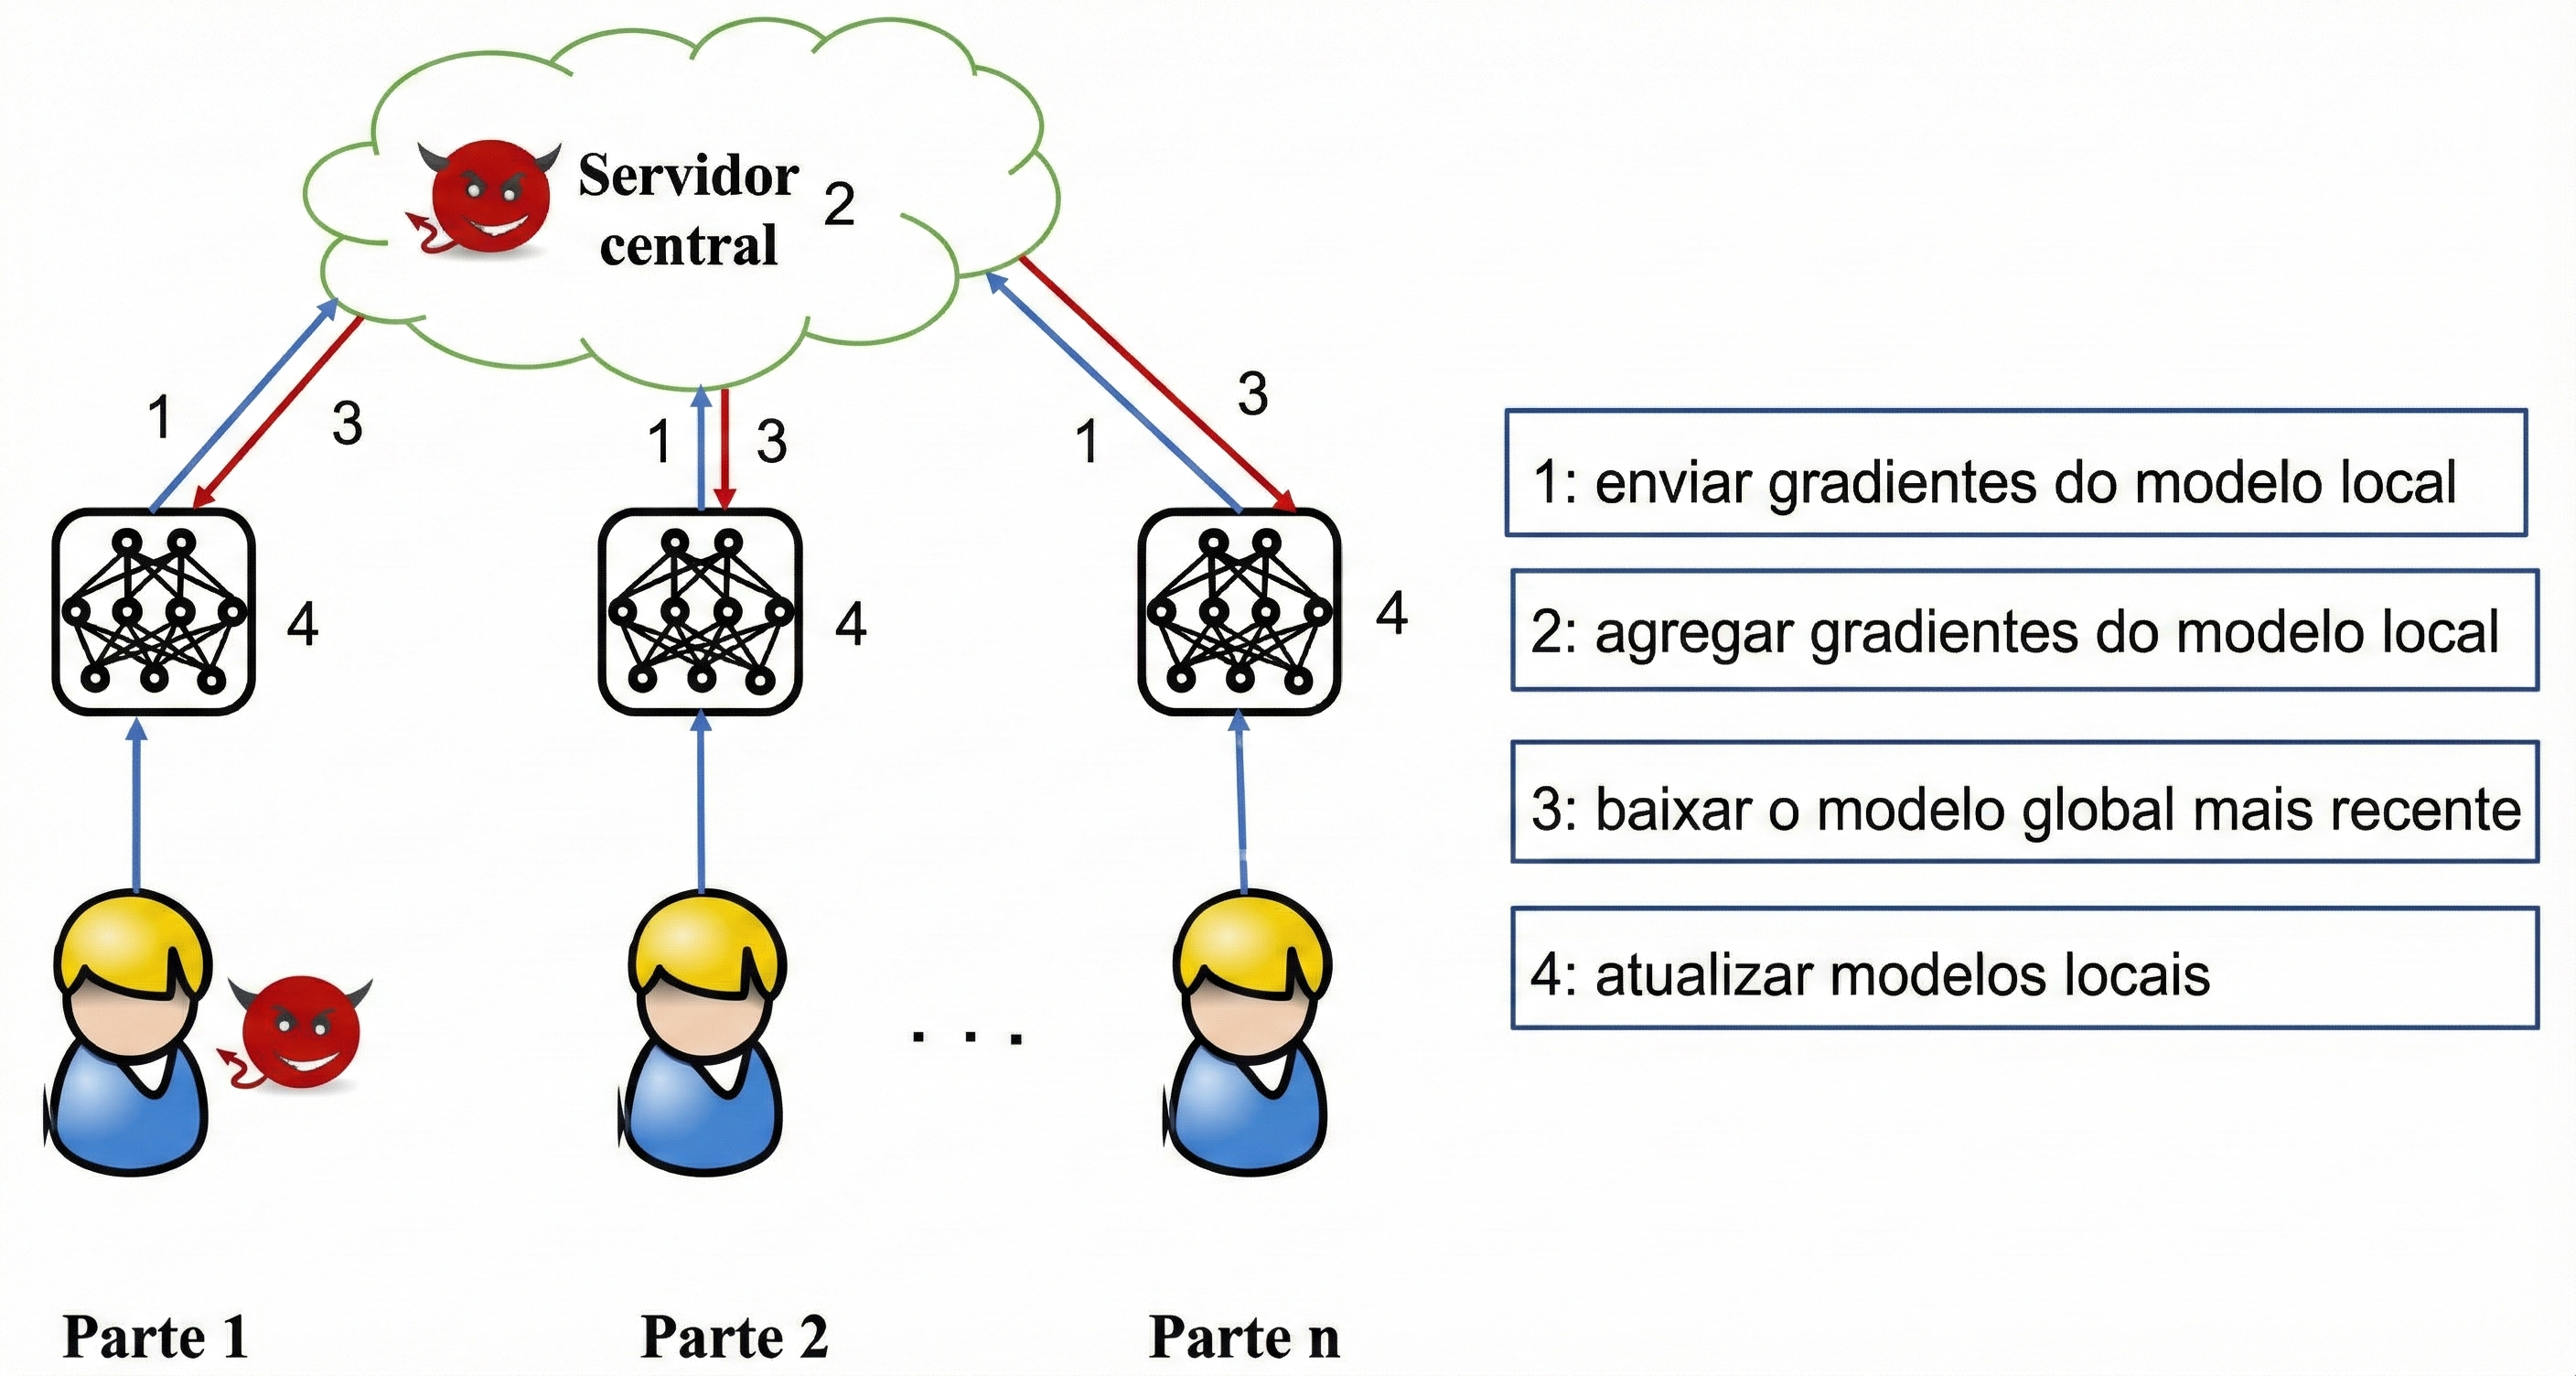
\includegraphics[width=0.9\textwidth]{figuras/poisoning-attack.png}
    \fonte{Adaptado de Lyu et al., 2020.}
    \label{fig:poisoning-attack}
\end{figure}


No ciclo ilustrado na Figura~\ref{fig:poisoning-attack}, um cliente pode inserir \textit{data poisoning} ao alterar dados locais antes do treinamento, ou \textit{model poisoning} ao manipular gradientes e parâmetros antes do envio. Ao processar atualizações contaminadas junto a contribuições benignas, o servidor pode atualizar o modelo global em direção adversa e, nas rodadas seguintes, propagar o modelo comprometido a todos os participantes \cite{Lyu2020}.

\subsection{Ataques em ambientes heterogêneos}
\label{subsec:ataques-heterogeneos}

A heterogeneidade estatística não \textit{IID} amplifica vulnerabilidades a ataques de \textit{poisoning}. Em cenários nos quais clientes detêm distribuições de dados significativamente distintas, contribuições maliciosas podem passar despercebidas ou exercer influência desproporcional, reduzindo a efetividade de mecanismos clássicos de agregação \cite{Zhao2018,Li2023}. Ataques persistentes, caracterizados pela atuação contínua de clientes maliciosos ao longo de múltiplas rodadas, podem levar a degradações cumulativas \cite{Tolpegin2020,Bhagoji2019}. Assim, defesas precisam considerar explicitamente a distribuição não uniforme de informações entre clientes, conforme discutido na Subseção~\ref{subsec:heterogeneidade-noniid} \cite{Mothukuri2021,Sikandar2023}.

\section{Estratégias de Defesa e Agregação Robusta}
\label{sec:defesa-agregacao-robusta}

Estratégias de defesa no \gls{fl} buscam mitigar ataques maliciosos durante a agregação de modelos locais. Esta seção apresenta algoritmos que serão objeto de avaliação experimental, incluindo métodos clássicos e abordagens modernas adaptativas.

\subsection{Métodos clássicos de agregação}
\label{subsec:metodos-classicos}

Algoritmos como \textit{Krum}, \textit{Trimmed Mean} e \textit{Median} são abordagens clássicas na literatura para defesa contra ataques bizantinos em \gls{fl} \cite{Blanchard2017,Yin2018}. O \textit{Krum} seleciona a atualização mais consistente com as demais, descartando \textit{outliers} \cite{Blanchard2017}, enquanto \textit{Trimmed Mean} e \textit{Median} removem valores extremos antes da agregação \cite{Yin2018}. Esses métodos assumem que atualizações maliciosas serão estatisticamente distantes das benignas e exploram propriedades geométricas e estatísticas das atualizações recebidas \cite{Blanchard2017,Yin2018}.

Entretanto, métodos clássicos podem sofrer degradação sob ataques sofisticados em ambientes não \textit{IID} \cite{Li2023,Chen2023}. Uma limitação recorrente é a dificuldade de distinguir heterogeneidade legítima de dados e comportamentos maliciosos quando a distribuição entre clientes é altamente heterogênea \cite{Li2023,Sikandar2023}.

A Tabela~\ref{tab:metodos-classicos} resume características dos métodos clássicos.

\begin{table}[htbp]
    \centering
    \caption{Comparação de métodos clássicos de agregação robusta}
    \label{tab:metodos-classicos}
    \begin{tabular}{lccc}
        \hline
        \textbf{Método} & \textbf{Princípio} & \textbf{Robustez} & \textbf{Complexidade} \\
        \hline
        \textit{Krum} & Seleção por proximidade & Moderada & Baixa \\
        \textit{Trimmed Mean} & Remoção de extremos & Moderada & Média \\
        \textit{Median} & Agregação por mediana & Baixa em \textit{Non-IID} & Baixa \\
        \hline
    \end{tabular}
    \fonte{Adaptado de Moshawrab et al., 2023.}
\end{table}

\subsection{Métodos modernos e adaptativos}
\label{subsec:metodos-modernos}

Abordagens modernas incorporam mecanismos de detecção de anomalias, matrizes de credibilidade dinâmica e técnicas de minimização de variância para superar limitações de métodos clássicos \cite{Chen2023,Xu2024}. O \textit{FLRAM} combina detecção de anomalias com uma matriz de credibilidade dinâmica que pondera a confiabilidade de cada cliente ao longo das rodadas, buscando robustez contra múltiplos tipos de ataque sem requerer conhecimento prévio do número de atacantes \cite{Chen2023}.

O \textit{MinVar} formula a defesa como minimização da variância ponderada das atualizações recebidas \cite{Xu2024}. Diferentemente de abordagens dicotômicas que aceitam ou rejeitam contribuições, o \textit{MinVar} atribui pesos contínuos às atualizações, permitindo contribuição de clientes honestos com dados não \textit{IID} mesmo quando suas atualizações são estatisticamente atípicas \cite{Xu2024}.

A Tabela~\ref{tab:comparacao-robustez} sintetiza uma comparação qualitativa de robustez reportada na literatura entre métodos clássicos e modernos sob diferentes condições adversariais.

\begin{table}[htbp]
    \centering
    \caption{Análise comparativa de robustez em métodos clássicos versus modernos}
    \label{tab:comparacao-robustez}
    \begin{tabular}{lccc}
        \hline
        \textbf{Método} & \textbf{Robustez IID} & \textbf{Robustez Non-IID} & \textbf{Múltiplos atacantes} \\
        \hline
        \textit{Krum}\textsuperscript{a} & Moderada & Fraca & Fraca \\
        \textit{Trimmed Mean}\textsuperscript{a} & Moderada & Fraca & Moderada \\
        \textit{Median}\textsuperscript{a} & Baixa & Muito fraca & Fraca \\
        \textit{FLRAM}\textsuperscript{b} & Forte & Forte & Forte \\
        \textit{MinVar}\textsuperscript{c} & Forte & Forte & Forte \\
        \hline
    \end{tabular}
    \fonte{Compilado pelo autor com base em: \textsuperscript{a}Blanchard et al., 2017 e Yin et al., 2018; \textsuperscript{b}Chen et al., 2023; \textsuperscript{c}Xu e Shu, 2024.}
\end{table}

\subsection{Abordagens híbridas: \textit{clustering} e minimização de variância}
\label{subsec:abordagens-hibridas}

O \textit{Mini-FL} introduz \textit{clustering} não supervisionado para agrupar atualizações antes da agregação robusta, com o objetivo de formar grupos com menor variância estatística e reduzir a superfície de ataque \cite{Li2023}. O \textit{MinVar} oferece perspectiva complementar ao minimizar variância ponderada, atribuindo pesos variáveis a todas as atualizações em vez de simplesmente aceitar ou descartar contribuições \cite{Xu2024}. O \textit{FLRAM} combina detecção de anomalias e credibilidade dinâmica para lidar com mudanças de comportamento ao longo do tempo \cite{Chen2023}.

A escolha entre essas abordagens depende do perfil de ataque esperado: \textit{clustering} tende a ser apropriado quando há diversidade de padrões entre clientes; minimização de variância busca robustez sob colusão (vários clientes adversários agindo de forma coordenada); matrizes de credibilidade oferecem adaptabilidade dinâmica ao longo das rodadas \cite{Chen2023,Li2023,Xu2024}.

\subsection{Métricas de avaliação experimental}
\label{subsec:metricas-avaliacao}

Para avaliar rigorosamente a efetividade de estratégias de defesa contra ataques adversariais, é necessário estabelecer métricas quantitativas que capturem múltiplos aspectos do desempenho \cite{Khan2023}. As principais métricas frequentemente utilizadas incluem:

\begin{itemize}
    \item \textbf{Acurácia do modelo global:} percentual de predições corretas em dados de teste, comparando o modelo sob ataque e o ambiente limpo \cite{Almutairi2024}.

    \item \textbf{Taxa de convergência:} número de rodadas necessárias para atingir um patamar de desempenho definido. Defesas que comprometem velocidade de convergência por descartes agressivos podem ser inviáveis quando comunicação é custosa \cite{Kairouz2021}.

    \item \textbf{Sobrecarga de comunicação:} quantidade total de dados trafegados entre clientes e servidor ao longo do treinamento. Métodos baseados em \textit{clustering} podem apresentar custos diferentes de abordagens criptográficas como \textit{Secure Multiparty Computation}, conhecida pela sigla \textit{SMPC} \cite{Moshawrab2023}.

    \item \textbf{Complexidade computacional:} tempo de processamento necessário no servidor para agregar atualizações recebidas, relevante em modelos com grande número de parâmetros \cite{Li2020}.
\end{itemize}

\subsection{Análise crítica: impacto da heterogeneidade}
\label{subsec:analise-critica-heterogeneidade}

A Tabela~\ref{tab:analise-heterogeneidade} resume dados reportados na literatura sobre impacto da heterogeneidade no desempenho de defesas em cenários \textit{Non-IID} \cite{Blanchard2017,Yin2018,Li2023,Xu2024}.


\begin{table}[H]
    \centering
    \caption{Impacto da heterogeneidade: acurácia de defesas em cenários \textit{Non-IID}}
    \label{tab:analise-heterogeneidade}
    \begin{tabular}{lccc}
        \hline
        \textbf{Método} & \textbf{MNIST IID} & \textbf{MNIST \textit{Non-IID} extremo} & \textbf{Robustez} \\
        \hline
        \textit{Krum}\textsuperscript{a} & 74,92\% & 44,15\% & Fraca \\
        \textit{Median}\textsuperscript{a} & 53,76\% & 2,85\% & Muito fraca \\
        \textit{Trimmed Mean}\textsuperscript{a} & 52,83\% & 8,36\% & Muito fraca \\
        \textit{Mini-Krum}\textsuperscript{b} & 89,62\% & 87,32\% & Forte \\
        \textit{Mini-Median}\textsuperscript{b} & 90,37\% & 89,77\% & Forte \\
        \textit{MinVar}\textsuperscript{c} & 92,15\% & 90,84\% & Forte \\
        \hline
    \end{tabular}
    \fonte{Compilado pelo autor com base em: \textsuperscript{a}Blanchard et al., 2017 e Yin et al., 2018; \textsuperscript{b}Li et al., 2023; \textsuperscript{c}Xu e Shu, 2024.}
\end{table}

A literatura indica que a efetividade de estratégias de defesa está ligada ao grau de heterogeneidade presente no ambiente \cite{Li2023,Xu2024}. Em cenários com distribuição extremamente heterogênea, métodos clássicos podem sofrer degradação acentuada, enquanto abordagens adaptativas tendem a manter desempenho mais estável \cite{Li2023}. Assim, a escolha de agregação robusta deve considerar explicitamente o perfil de heterogeneidade esperado nos dados dos clientes e o contexto de implantação \cite{Khan2023}.

A avaliação crítica também aponta questões metodológicas relevantes. Trabalhos recentes discutem se novas estratégias de agregação são estritamente necessárias ou se aprimoramentos em componentes conhecidos, como seleção de clientes e otimização de hiperparâmetros, podem alcançar robustez prática aceitável \cite{Fang2025}. Essas reflexões reforçam a necessidade de avaliações experimentais sistemáticas, sob condições controladas e realistas, para conclusões confiáveis sobre a efetividade de cada técnica \cite{Khan2023}.
